\documentclass[a4paper, 12pt]{ppgeb}

% |--- Títulos, autor, banca ---|----------------------{{{
% Autor:
% Substituta  as informações nos comandos a seguir, até a linha começando
% com \membrobancaexterno.
% Em \title: título na forma principal, como aparecerá em algumas páginas
% Em \tituloficha: título como aparecerá na ficha catalográfica; idêntico
% ao anterior, mas com possíveis quebras manuais de linha (usar \\ quando
% necessário, para ajustar as mudanças de linha na ficha catalográfica).
% Em   \titulocapaA,   \titulocapaB,   \titulocapaC:  título para a capa,
% dividido em no  máximo 3  linhas (coloque uma  linha em  cada  comando,
% dividindo como ficar melhor esteticamente).
% Remova  o  símbolo  de  comentário  (%)  de  \coorientador,  se  houver
% coorientador.
%  Em  \publicacao{011A/2019}:  o  número  final  será   fornecido   pela

\title{Coleta Simultânea de Eletroencefalograma \\ e Rastreamento Ocular: Ferramenta e Estudo de Caso}
\tituloficha{Coleta Simultânea de Eletroencefalograma e Rastreamento Ocular: Ferramenta e Estudo de Caso\\\phantom{}[Distrito Federal], 2019.} 
\titulocapaA{Coleta Simultânea de Eletroencefalograma e}
\titulocapaB{e Rastreamento Ocular: Ferramenta e Estudo de Caso}
\titulocapaC{}
\titulofichadois{Coleta Simultânea de Eletroencefalograma e Rastreamento Ocular: Ferramenta e Estudo de Caso}
\author{Ana Paula Sandes de Souza}
\nomeinvertido{Souza, Ana}
\orientador{Dr. Gerardo Antonio Idrobo Pizo}
%\coorientador{Nome do Coorientador}
\publicacao{011A/2022}
\data{Agosto de 2022}
\ano{2022}
\areaum{Neurociência Computacional} % Preencher com termos escolhidos para identificar a área
\areadois{Eletroencefalograma}
\areatres{Rastreamento Ocular}
\areaquatro{Sincronização de Sinais}
\endereco{anapaulasandes.s@gmail.com}
\cep{CEP 73105-904}

\membrobancainterno{DRª. Marília Miranda Forte Gomes}
\membrobancaexterno{Dr. Membro Externo}
%---}}}

% |--- Bibliotecas utilizadas ---|----------------------{{{
\usepackage[margin=1in]{geometry}
\usepackage{setspace}
\usepackage{multirow}
\usepackage{booktabs}
 \usepackage[brazil]{babel}
\usepackage{xfrac}
\usepackage{hyperref}
\hypersetup{
colorlinks = true,
linkcolor = black,
anchorcolor = blue,
citecolor = blue,
filecolor = blue,
urlcolor = blue
}
\usepackage{rotating}
\usepackage[margin=0.40in,font=small,labelfont=bf,labelsep=period]{caption}
%---}}}

% |- Formato de referências (use apenas uma das 2 linhas seguintes; comente a outra) -|-{{{
\newcommand{\formatobibliografia}{numero}
%\newcommand{\formatobibliografia}{autorano}

\ifthenelse{\equal{\formatobibliografia}{numero}}{
\bibliographystyle{plain}
}
{}

\ifthenelse{\equal{\formatobibliografia}{autorano}}{
\usepackage{apalike}
\bibliographystyle{apalike}
}
{}
%---}}}

% |--- Espaçamento, configuração de título de seções ---|----------------------{{{
\onehalfspacing

\makeatletter
\renewcommand{\section}{\@startsection
{section}
{1}
{0mm}
{-\baselineskip}
{0.5\baselineskip}
{\large\bfseries\scshape}}
\makeatother

\makeatletter
\renewcommand{\subsection}{\@startsection
{subsection}
{2}
{0mm}
{-\baselineskip}
{0.5\baselineskip}
{\bf\sffamily}}
\makeatother

\makeatletter
\renewcommand{\subsubsection}{\@startsection
{subsubsection}
{3}
{0mm}
{-\baselineskip}
{0.5\baselineskip}
{\bf\sffamily}}
\makeatother

\setlength{\parindent}{20pt}
\setlength{\parskip}{06pt}
\newcommand{\spaceinitialsname}{0.4mm}
\newcommand{\porcento}{\scalebox{0.5}{~}\scalebox{0.9}{\%}}
\newcommand{\scanner}{\emph{scanner}}
\newcommand{\scanners}{\emph{scanners}}
\newcommand{\cmcubico}{${\textrm{cm}^{\scalebox{0.7}{3} }}$}
\setcounter{secnumdepth}{3}
%\setcounter{tocdepth}{3}
%---}}}

% |--- Comandos especiais ---|----------------------{{{
\newcommand{\cmquad}{${\textrm{cm}^{\scalebox{0.7}{2}} }$}
\newcommand{\mmquad}{${\textrm{mm}^{\scalebox{0.7}{2}} }$}
\newcommand{\gcmquad}{${\textrm{g}}/{\textrm{cm}^{\scalebox{0.7}{2}} }$}
\newcommand{\subsecref}[1]{Seção~\ref{#1}}
\newcommand{\figref}[1]{Figura~\ref{#1}}
\newcommand{\etal}{\emph{et~al.}}
\newcommand{\Jawsonly}{{\emph{Jaws-Only}} }
\newcommand{\jawsonly}{{\emph{jaws-only}} }
\newcommand{\software}{\emph{software}}
\newcommand{\percentagesignscale}{0.8}
\newcommand{\percent}{\scalebox{\percentagesignscale}{~\%}}
\newcommand{\subsubsubsection}[1]{\vspace{16pt}\noindent\textbf{#1}\\[12pt]}
%---}}}

% |--- Diretório(s) com figuras (se desejar, inclua subdiretórios) ---|-------------{{{
\graphicspath{{figuras/}}
%---}}}

% |--- Lista de palavras que não podem ser separadas em sílabas ---|------------------{{{
\hyphenation{development results Commissioning possibility Philadelphia Devic Calculations Calculation Language}
%---}}}

% |--- Texto principal ---|----------------------{{{
\begin{document}

\maketitle

% Se desejar uma epígrafe, remova o % do início das próximas linhas (até ==============)
%\clearpage
%\hspace{1mm}
%
%\vfill
%
%\hspace{1mm}
%
%\begin{center}
%\emph{Epígrafe} \\
%Autor da epígrafe
%\end{center}
%
%\hspace{1mm}
%
%\vfill
%
%\hspace{1mm} 
% ==============

% Se desejar uma dedicatória, remova o % do início das próximas linhas (até ==============)
%\clearpage
%\hspace{1mm}
%
%\vfill
%
%\begin{flushright}
%\begin{itshape}
%Texto da dedicatória.
%\end{itshape}
%\end{flushright}
% ==============

% Se desejar incluir agradecimentos, remova o % do início das próximas linhas (até ==============)
% \clearpage
%\noindent{\bfseries{\maiusc{\large Agradecimentos}} }
%
%\vspace{24pt} Agradecimentos
%
%\noindent 
%\clearpage
% ==============

\newgeometry{bottom=0.8in, top=0.9in, left=0.9in, right=0.9in}

\noindent{\bfseries{\maiusc{\large Resumo}} }
\acresetall % Manter essa linha!
\vspace{12pt}

O eletroencefalograma (EEG) e o rastreamento ocular (ET - \textit{Eye Tracking}) são 
formas não-invasivas de se observar o comportamento do sistema nervoso através da coleta da atividade
neural e posicionamento ocular ao longo do tempo. Desta forma, são importantes ferramentas na construção de bases de dados fisiológicos. 
Bases de dados com mais de um tipo de dado fisiológico conferem vantagens a respeito
do uso em algoritmos classificatórios, apresentando uma maior acurácia do que algortimos treinados
com datasets unimodais.
Apesar das vantagens de uso, o acesso a estes datasets ainda é restrito devido ao custo
dos equipamentos e a complexidade da sincronização entre diferentes sensores.
O presente estudo tem por objetivo apresentar uma ferramenta construída a partir de equipamentos
comerciais que tem como \textit{output} um dataset multimodal de EEG e ET coletados simultaneamente.
É esperado que a ferramenta promova acessibilidade a datasets multimodais ao gerar uma coleta com 
equipamentos de baixo custo (relativo a equipamentos clínicos) e incentive o desenvolvimento de diferentes áreas de pesquisa que possam se beneficiar do acesso facilitado da coleta de dados fisiológicos. A ferramenta será 
avaliada a respeito de sua capacidade de sincronização de EEG e ET, e o dataset multimodal será utilizado para treinar algoritmos 
classificatórios no software Orange em um estudo de caso com apresentação de estímulos emocionais durante o momento de coleta.
A performance dos algortimos será utilizada para argumentar sobre a possível aplicabilidade da ferramenta em estudos futuros.

\vspace{14pt}

\noindent{\textbf{Palavras-chave: }} EEG; ET; Sincronização; Base de Dados Fisiológicos;
\acresetall % Manter essa linha!
\clearpage
\restoregeometry
% \chapter{Abstract}
\noindent{\bfseries{\maiusc{\large Abstract}} }
\acresetall % Manter essa linha!
\vspace{24pt}

Electroencephalogram (EEG) and eye tracking (ET) are non-invasive ways of observing the nervous system behavior and are important tools in the construction of physiological databases. The equipment cost and synchronization of data are bottlenecks in the multimodal dataset construction. Studies relate physiological data integration to a higher classification accuracy in supervised learning algorithms. This study observes the latest methods of synchronizing data for building multimodal EEG and ET datasets trough the usage of commercially available equipment. It is expected that an affordable way of building multimodal databases will encourage the development of new machine learning algorithms, and increase the amount of physiological datasets available for future studies.

\vspace{14pt}

\noindent{\textbf{Keywords: }} EEG; ET; Synchronization; Physiological Dataset;
\acresetall % Manter essa linha!

\indice

\begin{center}

{\bfseries{\maiusc{\large Lista de Nomenclaturas e Abreviações}} }%
\end{center}

\acrodef{3DCRT}[3DCRT]{Radioterapia Conformacional 3D, do inglês \emph{3D Conformal Radiotherapy}}
\acrodef{AAPM}[AAPM]{Associação Americana de Física na Medicina, do inglês \emph{American Association of Physics in Medicine}}
\acrodef{CQ}[CQ]{Controle de Qualidade}
\acrodef{SPT}[SPT]{Sistema de Planejamento de Tratamento}

\begin{acronym}
\acro{3DCRT}{Radioterapia Conformacional 3D, do inglês \emph{3D Conformal Radiotherapy}}
\acro{AAPM}{Associação Americana de Física na Medicina, do inglês \emph{American Association of Physics in Medicine}}
\acro{CQ}{Controle de Qualidade}
\acro{SPT}{Sistema de Planejamento de Tratamento}
\end{acronym}

\clearpage

\pagenumbering{arabic}

\acresetall % Manter essa linha!

\chapter{Introdução}

Existe uma importante vantagem advinda do uso de bases fisiológicas chamadas multimodais, ou de mais de um tipo de dado fisiológico em algoritmos supervisionados: a possibilidade de conferir um maior poder classificatório em relação aos datasets unimodais (Kang et al., 2020; Thapaliya et al., 2019). Sobre os benefícios já alcançados com estes datasets, é possível citar: melhora de diagnóstico de transtornos neurológicos, como depressão e autismo (Kang et al., 2020; Thapaliya et al., 2019; Wu et al., 2021), maior poder de classificação de emoções (Guo et al., 2019; Zheng et al., 2019;  Lu et al, 2015; Zheng et al., 2014), e uma maior compreensão da ativação de mecanismos nervosos durante atividades de rotina, como leitura (Hollenstein et al., 2018). Um modelo específico de dataset fisiológico multimodal é constituído do eletroencefalograma (EEG) e rastreamento ocular (RO ou ET, da palavra em inglês Eye Tracking). Seu uso no treinamento de algoritmos classificatórios atestou sua aplicabilidade em diferentes contextos clínicos e acadêmicos, além de um aumento de acurácia na classificação de diferentes doenças nervosas e de emoções. 

%Se você deseja que o primeiro parágrafo de cada seção também tenha indentação, inclua no preâmbulo o comando \verb,\usepackage{indentfirst},.

\section{Contextualização de Problema}

Apesar das múltiplas vantagens, o acesso a estes datasets ainda é restrito. Sobre a coleta de EEG e ET, Kastrati et al. (2021) comenta:


\textit{“Coletar e classificar dados simultâneos de EEG e de rastreamento ocular é demorado e caro, pois requer equipamento e experiência para aquisição de EEG e rastreamento ocular. Portanto, o acesso a dados de EEG-ET gravados simultaneamente é altamente restrito, o que retarda significativamente o progresso neste campo”. – Kastrati et al. (2021).}

A redução do custo das coletas fisiológicas já vem sido abordada através de equipamentos comercialmente disponíveis. Um exemplo é o desenvolvimento de “smart watches”, pequenos computadores de pulso que permitem o acompanhamento da frequência cardíaca do usuário, além do monitoramento de outras atividades fisiológicas, como o sono. O Mindwave Mobile 2, do fabricante Neurosky®, é um exemplo de equipamento comercial que possibilita a captura de ondas cerebrais e métricas próprias do fabricante utilizadas para estimar medidas de atenção, meditação e a captura de piscadas dos usuários. Este equipamento permite o desenvolvimento de aplicações na forma de jogos interativos, neurofeedback e outras aplicações lúdicas (Neurosky). A respeito de seu uso em pesquisas científicas, ele já foi utilizado para estimar quais métodos de ensino despertavam maior atenção em alunos do ensino fundamental, estimar personalidade de participantes através da apresentação de vídeo clips eleitos para instigar um determinado traço de personalidade, e classificação de emoções. Além deste equipamento para coleta de EEG, também existem equipamentos disponíveis comercialmente para a coleta de ET, como o GP3 (Gazepoint®). 


Com o propósito de aumentar a acessibilidade aos datasets multimodais e suas amplas vantagens de uso, o presente projeto tem por objetivo a criação de uma ferramenta de coleta simultânea de EEG e RO acessível a partir da coleta de dados de dois equipamentos comerciais – GP3 para a coleta de RO, e Mindwave Mobile 2 para a coleta de dados de ativação neuronal. A ferramenta terá como output um dataset constituído de dados de EEG e RO coletados simultaneamente. O output será testado em um estudo de caso através da análise de performance de quatro diferentes algoritmos classificatórios treinados com o output para classificar entre duas possíveis atividades. 


\section{Objetivos}

Criar uma ferramenta capaz de gerar um dataset de EEG e ET coletado de forma síncrona e validar o dataset através da performance de algoritmos de aprendizado supervisionado treinados com ele.

\subsection{Objetivos Específicos}

\begin{enumerate}
    \item Criar código para coleta simultânea de EEG e RO;
    \item Criar dataset multimodal a partir da fusão de dados de EEG e RO coletados pela ferramenta e classificado de acordo com o estímulo apresentado ao participante;
    \item Treinar diferentes algoritmos supervisionados com o dataset multimodal gerado;
\end{enumerate}

\section{Justificativa}
Apesar da existência de técnicas que permitam a extração de mais de um modo de dados fisiológicos a partir de um equipamento apenas - como a extração da posição ocular a partir de assinaturas elétricas em dados de EEG, estes métodos necessitam de um grande volume de dados, o que exige equipamentos mais refinados e, por vezes, uma grande disponibilidade de tempo para criação dos datasets e deslocamento de participantes até a estação de coleta. A coleta de ET e EEG por equipamento comercial e acessível, seria, portanto, uma alternativa que permite um maior controle no desenvolvimento de estudos com algoritmos de aprendizado de máquina, sem depender de equipamentos de alto custo ou deslocamento de participantes até a estação. 


É argumentado que um maior acesso a construção de bases de dados multimodais poderá expandir e aprofundar os avanços em neurociência e estudos comportamentais, ao proporcionar um maior controle do design de experimento e expandir a quantidade de datasets fisiológicos gerados. 

\section{Organização do Documento}
O presente texto tem nove capítulos. O primeiro capítulo trata da contextualização do problema, objetivos gerais e específicos, e a justificativa para a abordagem selecionada. 

O segundo capítulo trata do referencial teórico, levantando pontos históricos importantes ao desenvolvimento desta pesquisa, uma introdução ao que seriam os sinais capturados pelos dois equipamentos de EEG e ET, características dos diferentes tipos de equipamento de captura e aborda a conversão de sinais analógicos para digital. 

O terceiro capítulo trata do processo da aquisição e do tratamento de sinais fisiológicos a serem classificados por algoritmos de aprendizado de máquina supervisionado – processos como remoção de ruído e seleção de características. Também aborda métodos de fusão de bases de dados de diferentes fontes - a nível de característica e a nível de decisão. 

O quarto capítulo apresenta os métodos de avaliação dos algoritmos classificatórios. 

O quinto capítulo aprofunda nos possíveis métodos de sincronização de coleta e de bases de dados.

O sexto capítulo introduz a proposta de ferramenta de coleta simultânea elaborada por código e aborda o método de sincronização off-line, com sincronização por código temporal. 

O sétimo capítulo aborda o cronograma.

O oitavo capítulo aborda os resultados esperados do estudo.


O nono capítulo apresenta as referencias do estudo.

\chapter{Eletricidade Cerebral}



\section{Correntes Elétricas}
%Gaspar, Alberto (2005). Física:Volume único. São Paulo: Editora Ática. 496 páginas. ISBN 9788508078837. Consultado em 12 de janeiro de 2012
A eletricidade é o nome dado a uma série de fenômenos que envolvem o fluxo de cargas elétricas (Gaspar, 2005). 
O potencial elétrico (também conhecido como tensão), é a quantidade de energia precisa para deslocar uma carga elétrica (Matias e Fratezzi, 2008). 
A diferença de potencial elétrico entre um material condutor gera um fluxo de 
cargas nomeado de \textbf{corrente elétrica} (Creder, 1989).
A intensidade do fluxo é medida em ampère (A) e determinada pela quantiadade de partículas que atravessam o seguimento
do condutor pelo tempo. As correntes podem ser contínuas ou alternadas, a depender se o sentido da corrente varia ou não; enquanto a corrente contínua 
é composta de polos, a alternada é composta de fases (Bhargava e Kulshreshtha, 1983). O calculo de corrente elétrica é 
dado pela seguinte equação:

\begin{equation}
    I = \frac{\Delta Q }{\Delta T},
\end{equation}

onde $\Delta Q$ é a quantidade de particulas que passam em um seguimento do condutor e $\Delta T$ indica o tempo. 

\section{Neurônios}
Os neurônios são células responsáveis pela condução de impulsos nervosos e se comportam como um “cabo eletrificado” - analogia
levantada a respeito da condução de impulsos elétricos, como apresentado no clássico estudo de Hodgkin e Huxley (1952), 
que teve como resultado uma modelagem dos potenciais de ação emitidos pelas células 
nervosas através de equações diferenciais não-lineares (figura 2.2). 
Os neurônios comunicam-se uns com os outros através das \textbf{sinapses}, onde ocorre a transmissão dos impulsos nervosos. 
É possível distinguir três partes anatomicas no neurônio: o corpo celular, o axônio e os dendrito (figura 2.1). 

\begin{figure}
    \centering
    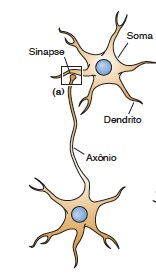
\includegraphics[width=40mm]{corpo_celular.jpg}
    \caption{Anatomia de um neurônio com destaque para área de sinapse entre neurônios. Fonte: Bear (2015)}
\end{figure}

% Serway, R.A.; Jewett Jr., J.W (2008). Princípios de Física. 3. São Paulo: Cengage Learning. p. 909-910. ISBN 85-221-0414-X
A membrana celular permite a passagem de cargas elétricas através de canais, que podem ou não necessitar de energia para a movimentação
das cargas. \textbf{Capacitores} são dispositivos de polaridades diferentes nas extremidades, que armazenam
cargas elétricas num campo elétrico (Serway, 2008). Por sua capacidade de separar cargas elétricas entre o ambiente interno e externo, 
a membrana celular age como os capacitadores, com sua capacitância (habilidade de armazenar cargas elétricas), definida pela seguinte equação:

\begin{equation}
    C = \frac{Q}{\Delta V},
\end{equation}

onde $C$ é a capacitância, $Q$ é a quantidade de carga armazenada e $\Delta V$ é a tensão elétrica, medida em farad (F). 
\textbf{Resistência elétrica} diz respeito a capacidade de oposição a passagem de corrente elétrica e é medido em
 ohms ($\Omega$). Os canais da membrana podem se comportar como resistores, se opondo a passagem da corrente elétrica, e sua 
 resistencia pode variar dependendo das condições celulares, como por exemplo se o canal está abero ou  não. Na figura 2.2, $E$ representa
 \textbf{bateria} pois a concentração de ions (particulas elétricas) é diferente no meio intra e extracelular, graças ao trabalho de canais ativos (com custo de energia
 para manter esse diferencial). De forma simplificada, a corrente aplicada no neurônio pode injetar corrente no capacitor e também 
 ser distribuída pelos canais. Dado a definição de um capacitor, $I_c = d u /d t$, é possível definir a corrente elétrica em uma seção da 
 membrana como:


%https://neuronaldynamics.epfl.ch/online/Ch2.S2.html#Ch2.F2
\begin{figure}
    \centering
    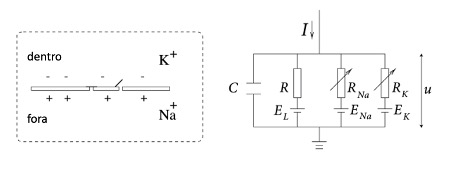
\includegraphics[width=100mm]{modeloHH.jpg}
    \caption{Esquema Modelo Hodgkin-Huxley. 
    Dentro: indicando espaço intracelular; fora: indicando espaço extracelular (imagem a esquerda). Direita: 
    C = capacitor, R = resistor, E = Baterias. Na = Sódio, K = Potássio  Fonte: Neuromal Dynamcs (2014)} 
\end{figure}

\begin{equation}
    C \frac{d u }{ d t} =  - \sum_{k} I_k (t) + I (t),
\end{equation}

onde $u$ = voltagem ao longo da membrana e $t$ = tempo. 




\subsection{Impulsos Nervosos e Potencial de Ação}
Para passar informações, os neurônios geram \textbf{impulsos nervosos}, ou alterações no potencial elétrico de sua membrana. Este sinal elétrico
ocorre quando o estímulo recebido pelo neurônio ultrapassa um limiar de ativação, que desencadeia uma série de respostas celulares. A célula pode 
estar em repouso (com valor do interior celular em cerca de -70mV), passando por despolarização (quando ocorre um fluxo de cargas elétricas que faz com 
que o meio intracelular passe a ser positivo em relação ao meio extracelular), e em repolarização, quando a célula está retornando ao potencial de repouso,
como representado na figura 2.3. 

O aumento do inicial da voltagem é causado pela entrada de sódio através de canais dependentes de voltagem, que se segue 
pela perda de potássio e fechamento dos canais de sódio. 


\begin{figure}[!h]
    \centering
    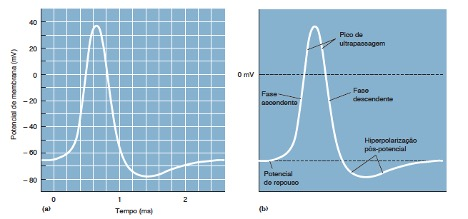
\includegraphics[width=120mm]{potencial_de_membrana_bear.jpg}
    \caption[Impulsos nervosos conduzidos em neurônios]{Resumo do potencial de ação. Fonte: Bear (2015).}.\label{fig:potencial}
    \end{figure}


\section{Eletroencefalograma}
O conjunto de impulsos nervosos de grupos de neurônios geram campos
magnéticos que podem ser captados por eletrodos colocados sobre a cabeça humana
(Kandel, 2000). Estes campos magnéticos foram primeiro registrados de coletas em
humanos aproximadamente em 1929, em um experimento conduzido pelo psiquiatra
alemão Hans Berger (Ince et al., 2021) – figura
2.4. Estes registros são o resultado dos potenciais de ação emitidos pelas células
nervosas abaixo do eletrodo, e permitem uma boa resolução temporal do
comportamento nervoso (podendo atingir precisão de milissegundos), mas em geral
não permitem uma boa resolução espacial (como identificar a localização espacial do
grupo celular responsável pela variação de voltagem observada).

  \begin{figure}[h]
    \centering
    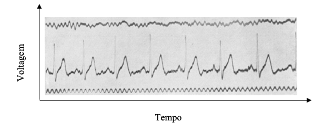
\includegraphics[width=100mm]{serie_temporal_EEG}
    \caption[]{Primeiro EEG registrado em humanos, resultado do trabalho do psiquiatra Hans Berger. Fonte: Ince et al. (2021).} 
    \end{figure}

\section{Ondas Cerebrais}
% Llinas, R. R. (2014). "Intrinsic electrical properties of mammalian neurons and CNS function: a historical perspective". Front Cell Neurosci. 8: 320. doi:10.3389/fncel.2014.00320. PMC 4219458free to read. PMID 25408634
O cérebro consegue gerar ondas ritmicas geradas pelos impulsos nervosos de grupos de neurônios. 
A oscilação de um neurônio único pode ser explorada na figura 2.3. As grandes oscilações (geradas por 
mais de um nerônio sendo ativado) pode ser detectada pelos eletrodos posicionados 
no crânio no eletroencefalograma (Llinas, 2014) e serem classificadas de acordo com suas características.
Um exemplo de agrupamento das ondas cerebrais pode ser observado na figura 2.5. 

\begin{figure}[h]
    \centering
    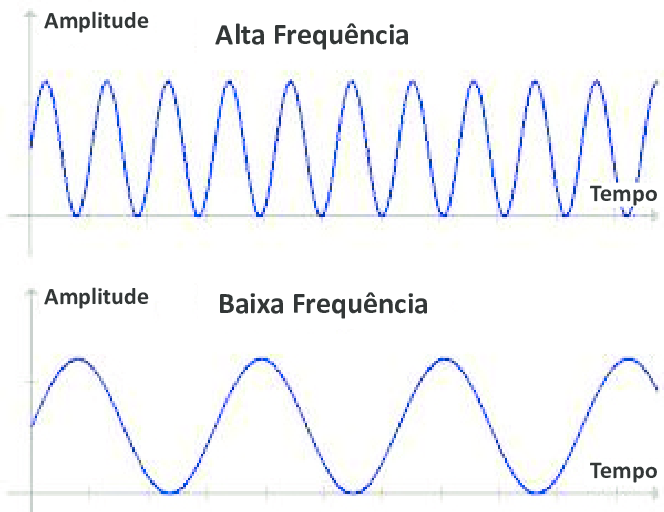
\includegraphics[width=100mm]{propriedades de onda.png}
    \caption[]{Representação das propriedades de onda.} 
    \end{figure}

As ondas cerebrais são caracterizadas pela \textbf{frequência, amplitude e fase} (figura 2.5). 
A amplitude mede a magnitude da oscilação de uma onda e pode ser representada pela equação

\begin{equation}
    y = A * sen (t - k) + b,
\end{equation}
onde $y$ é a função de onda (mede amplitude no instante t), $A$ é a amplitude da onda, sen representa
uma função senoidal, $t$ é o tempo, $k$ é a transalação temporal e b mede a translação de onda. 

\begin{figure}[h]
    \centering
    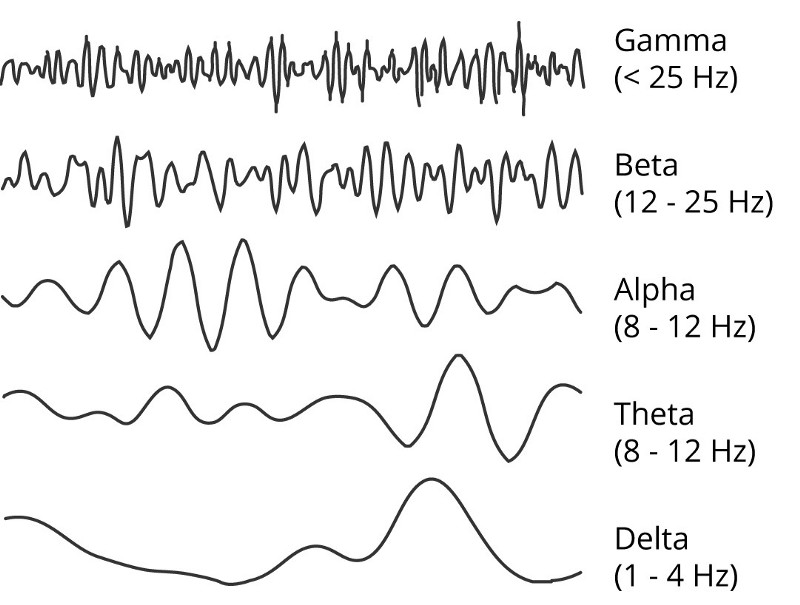
\includegraphics[width=80mm]{1_smvgacGqEOqIoKmjhzbfPw.jpeg}
    \caption[]{Ondas gamma, beta, alfa, teta e delta.} 
    \end{figure}


\subsection{Sistema Internacional 10/20 de Posicionamento de Eletrodos} 

    A técnica de registro de EEG vem sendo desde então aperfeiçoada e escolhida em
    investigações comportamentais devido a sua natureza não invasiva. Um exemplo de
    aperfeiçoamento foi a criação de um sistema internacional de posicionamentos de
    eletrodos para a coleta de EEG – o sistema 10/20 (Klem et al., 1999), 
    representado na figura 2.6.
    O registro capturado nos eletrodos
    advém de uma diferença de potencial elétrico. Esta diferença pode ser em referência à
    um eletrodo colocado em uma região externa ao escalpo (como orelha), ou à uma
    voltagem média comum (Tavares, 2011).


\begin{figure}[h]
    \centering
    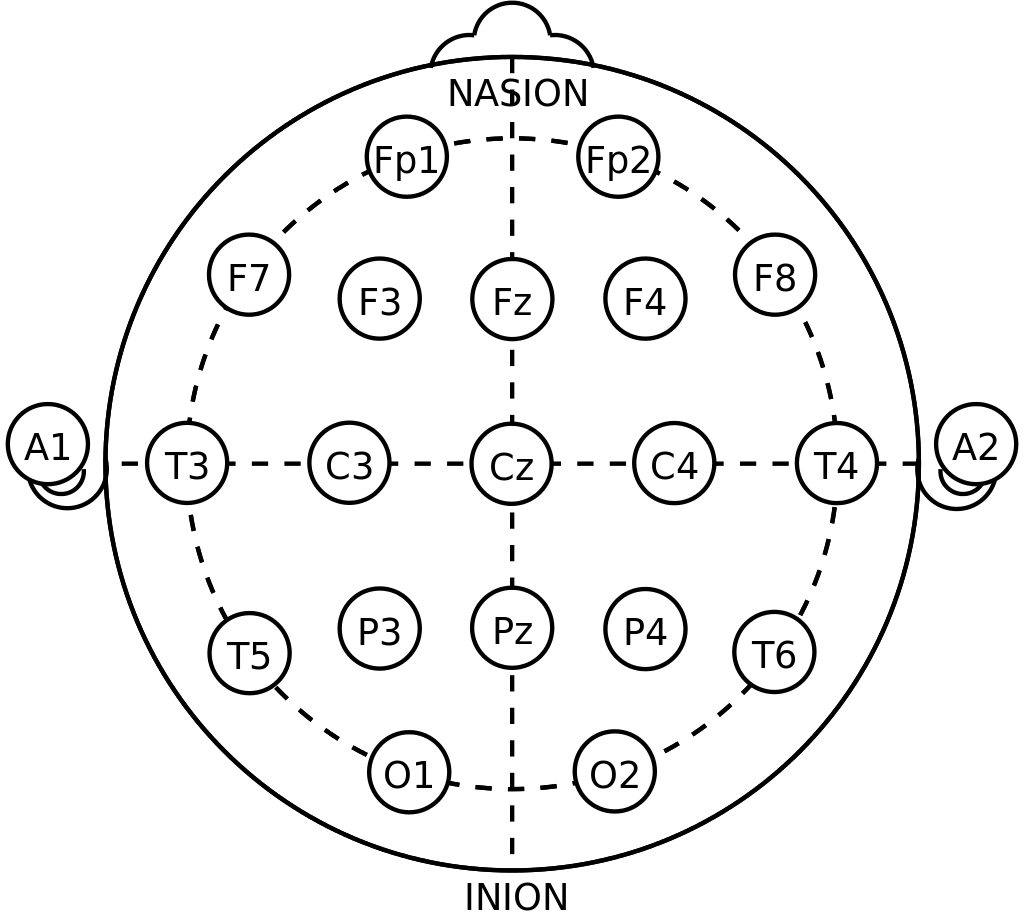
\includegraphics[width=100mm]{21_electrodes_of_International_10-20_system_for_EEG.png}
    \caption[]{Sistema Internacional 10/20 de Posicionamento de Eletrodos. Em destaque:
    Posição do eletrodo de coleta passiva do MindWave Mobile 2. A = Ear lobe, AF = anterior
    frontal, C = central, CP = centroparietal, F = frontal, FC = frontocentral, FT =
    frontotemporal, N = nasion, O = occipital, P = parietal, PO = parietooccipital, T = temporal.
    
    Klem et al. (1999).} 
    \end{figure}
    
    
        
\subsection{Tipos de Eletrodos para Captura de EEG}

    Existem diferentes tipos de eletrodos para a captura de EEG. 
    Um resumo é apresentado no quadro 2.1. É notável também que com o 
    desenvolvimento da capacidade computacional, novos recursos e métodos 
    para a análise destes dados vem sendo benéficos à construção do conhecimento 
    científico, agora também contando com o desenvolvimento de algoritmos de aprendizado
     de máquina, aprendizado profundo e inteligência artificial. 

     \begin{quadro}
        \caption{Tipos de Eletrodos para coleta de EEG (adaptado de Brain Support Inc. (2019)):}\label{quadro:exemplo}
        \begin{center}
        \scalefont{0.905}
        \begin{tabular}{|l|l|}
        \hline
        \hfill Tipo de Eletrodo\hfill\hspace{1mm} & \hfill Descrição\hfill\hspace{1mm}\\
        \hline
        Passivo &  \hspace{-06pt}\begin{tabular}{l}Geralmente feitos de prata, contam com a aplicação 
            de gel condutor \\
        para reduzir a perda de informação antes de serem colocados \\ na cabeça do participante.\end{tabular}\\
        \hline
        Ativo & \hspace{-06pt}\begin{tabular}{l}Geralmente feitos em prata, permitem o registro de \\
            variações de voltagem com redução de ruído do ambiente \\
            através de um circuito integrado aos eletrodos, com \\
            conversores de impedância.\end{tabular}\\
        \hline
        Seco & \hspace{-06pt}\begin{tabular}{l}Não necessita da aplicação de gel 
            para melhora da coleta do sinal.\end{tabular}\\
        \hline
        \end{tabular}
        \scalefont{1.4184}
        \end{center}
        \vspace{-12pt}
        Fonte: Brain Support Inc. (2019).\\
        \end{quadro}
        
  

    % Please add the following required packages to your document preamble:
% Please add the following required packages to your document preamble:
% \usepackage{graphicx}



%\subsection{Potenciais Relacionados a Eventos}




\chapter{Captura de Rastreamento Ocular}

\section{Anatomia Ocular}
O globo ocular é majoritariamente opaco, com exceção da córnea, que é transparente. 
A pupila é a região que da passagem para a luz e possui diâmetro variável. Os músculos da íris são os que controlam a dilatação da pupila. 
A focalização da imagem deve se concentrar na fóvea, onde se encontram células muito sensíveis a luz (Helene e Helene, 2011). 
A fixação ocular compreende a um período de cerca de 100 milissegundos onde o olhar se fixa em um ponto de convergência (Barreto et al., 2012). 
Este período se encerra com o movimento de sacada, que compreende ao movimento rápido até uma nova fixação do olhar em outro local.
Através da coleta do posicionamento ocular, é possível calcular uma taxa de dispersão focal ao longo do tempo e piscadas. 
Estes dados foram previamente correlacionados com estados emocionais (Soleymani et al., 2012) e 
também aplicados em estudos com algoritmos de aprendizado de máquina e deep learning. Barreto (2012)
resumiu alguns dos principais termos utilizados em pesquisas de rastreamento ocular (RO):

\section{Equipamentos de Rastreamento}
Para detectar onde o participante está focando seu olhar ao longo do tempo, alguns equipamentos de ET
 fazem uso de luz infravermelha e câmeras de alta definição que projetam a luz
  diretamente no olho do participante e gravam a direção do olhar a partir do reflexo. 
  Como a luz infravermelha abrange um comprimento de onda não detectável pelo olho humano, 
  o direcionamento desta luz no olho não interfere visão do participante. 
  O cálculo do direcionamento ocular é feito com base em algoritmos próprios de cada fabricante. 
  Existem alguns tipos de equipamentos de rastreamento ocular. São eles: (1) Webcam, (2) Vestível (Werable) e (3) Baseados em Tela. 
  Webcam diz respeito a equipamentos não especializados para o uso de rastreamento; usáveis correspondem a equipamentos como óculos de rastreamento ocular 
  e realidade virtual, e os baseados em tela dizem respeito aos equipamentos de coleta especializada que podem ser acoplados a um computador Tobii Pro (2020).

  \section{Calibração do Equipamento de Coleta}
  Como funciona a calibração

\chapter{Séries Temporais}

Séries temporais são sequencias de informações ao longo do tempo, onde informações vizinhas são dependentes (Ehlers, 2007). 
As séries podem ser contínuas ou discretas. Um exemplo de sinal contínuo é a diferença da voltagem de neurônios
capturada por eletrodos ao longo do tempo. Exemplos de séries temporais incluem:
\begin{itemize}
    \item Mudança de temperatura ao longo do dia
    \item Frequencia de Disparo de Neuronios ao longo do tempo
    \item Mudança de Voltagem ao longo do tempo 
\end{itemize}

As séries temporais tem um vasto uso em estatística, economia, matemática, entre outras áreas. 

Time series analysis comprises methods for analyzing time series data in order to extract meaningful statistics and other characteristics of the data.
 Time series forecasting is the use of a model to predict future values based on previously observed values. 
 While regression analysis is often employed in such a way as to test relationships between one or more different time series,
  this type of analysis is not usually called "time series analysis", 
  which refers in particular to relationships between different points in time within a single series. 
  Interrupted time series analysis is used to detect changes in the evolution of a time series from before 
  to after some intervention which may affect the underlying variable.

Time series data have a natural temporal ordering. This makes time series analysis distinct from cross-sectional studies, in which there is no natural ordering of the observations (e.g. explaining people's wages by reference to their respective education levels, where the individuals' data could be entered in any order). Time series analysis is also distinct from spatial data analysis where the observations typically relate to geographical locations (e.g. accounting for house prices by the location as well as the intrinsic characteristics of the houses). A stochastic model for a time series will generally reflect the fact that observations close together in time will be more closely related than observations further apart. In addition, time series models will often make use of the natural one-way ordering of time so that values for a given period will be expressed as deriving in some way from past values, rather than from future values (see time reversibility).

Time series analysis can be applied to real-valued, continuous data, discrete numeric data, or discrete symbolic data (i.e. sequences of characters, such as letters and words in the English language[1]).

Methods for analysis
Methods for time series analysis may be divided into two classes: frequency-domain methods and time-domain methods. The former include spectral analysis and wavelet analysis; the latter include auto-correlation and cross-correlation analysis. In the time domain, correlation and analysis can be made in a filter-like manner using scaled correlation, thereby mitigating the need to operate in the frequency domain.

Additionally, time series analysis techniques may be divided into parametric and non-parametric methods. The parametric approaches assume that the underlying stationary stochastic process has a certain structure which can be described using a small number of parameters (for example, using an autoregressive or moving average model). In these approaches, the task is to estimate the parameters of the model that describes the stochastic process. By contrast, non-parametric approaches explicitly estimate the covariance or the spectrum of the process without assuming that the process has any particular structure.

Methods of time series analysis may also be divided into linear and non-linear, and univariate and multivariate.

Panel data
A time series is one type of panel data. Panel data is the general class, a multidimensional data set, whereas a time series data set is a one-dimensional panel (as is a cross-sectional dataset). A data set may exhibit characteristics of both panel data and time series data. One way to tell is to ask what makes one data record unique from the other records. If the answer is the time data field, then this is a time series data set candidate. If determining a unique record requires a time data field and an additional identifier which is unrelated to time (e.g. student ID, stock symbol, country code), then it is panel data candidate. If the differentiation lies on the non-time identifier, then the data set is a cross-sectional data set candidate.

Analysis
There are several types of motivation and data analysis available for time series which are appropriate for different purposes.

Motivation
In the context of statistics, econometrics, quantitative finance, seismology, meteorology, and geophysics the primary goal of time series analysis is forecasting. In the context of signal processing, control engineering and communication engineering it is used for signal detection. Other applications are in data mining, pattern recognition and machine learning, where time series analysis can be used for clustering,[2][3] classification,[4] query by content,[5] anomaly detection as well as forecasting.[6]

Exploratory analysis

Tuberculosis incidence US 1953-2009
Further information: Exploratory analysis
A straightforward way to examine a regular time series is manually with a line chart. An example chart is shown on the right for tuberculosis incidence in the United States, made with a spreadsheet program. The number of cases was standardized to a rate per 100,000 and the percent change per year in this rate was calculated. The nearly steadily dropping line shows that the TB incidence was decreasing in most years, but the percent change in this rate varied by as much as +/- 10%, with 'surges' in 1975 and around the early 1990s. The use of both vertical axes allows the comparison of two time series in one graphic.

A study of corporate data analysts found two challenges to exploratory time series analysis: discovering the shape of interesting patterns, and finding an explanation for these patterns.[7] Visual tools that represent time series data as heat map matrices can help overcome these challenges.

Other techniques include:

Autocorrelation analysis to examine serial dependence
Spectral analysis to examine cyclic behavior which need not be related to seasonality. For example, sunspot activity varies over 11 year cycles.[8][9] Other common examples include celestial phenomena, weather patterns, neural activity, commodity prices, and economic activity.
Separation into components representing trend, seasonality, slow and fast variation, and cyclical irregularity: see trend estimation and decomposition of time series
Curve fitting
Main article: Curve fitting
Curve fitting[10][11] is the process of constructing a curve, or mathematical function, that has the best fit to a series of data points,[12] possibly subject to constraints.[13][14] Curve fitting can involve either interpolation,[15][16] where an exact fit to the data is required, or smoothing,[17][18] in which a "smooth" function is constructed that approximately fits the data. A related topic is regression analysis,[19][20] which focuses more on questions of statistical inference such as how much uncertainty is present in a curve that is fit to data observed with random errors. Fitted curves can be used as an aid for data visualization,[21][22] to infer values of a function where no data are available,[23] and to summarize the relationships among two or more variables.[24] Extrapolation refers to the use of a fitted curve beyond the range of the observed data,[25] and is subject to a degree of uncertainty[26] since it may reflect the method used to construct the curve as much as it reflects the observed data.

The construction of economic time series involves the estimation of some components for some dates by interpolation between values ("benchmarks") for earlier and later dates. Interpolation is estimation of an unknown quantity between two known quantities (historical data), or drawing conclusions about missing information from the available information ("reading between the lines").[27] Interpolation is useful where the data surrounding the missing data is available and its trend, seasonality, and longer-term cycles are known. This is often done by using a related series known for all relevant dates.[28] Alternatively polynomial interpolation or spline interpolation is used where piecewise polynomial functions are fit into time intervals such that they fit smoothly together. A different problem which is closely related to interpolation is the approximation of a complicated function by a simple function (also called regression). The main difference between regression and interpolation is that polynomial regression gives a single polynomial that models the entire data set. Spline interpolation, however, yield a piecewise continuous function composed of many polynomials to model the data set.

Extrapolation is the process of estimating, beyond the original observation range, the value of a variable on the basis of its relationship with another variable. It is similar to interpolation, which produces estimates between known observations, but extrapolation is subject to greater uncertainty and a higher risk of producing meaningless results.

Function approximation
Main article: Function approximation
In general, a function approximation problem asks us to select a function among a well-defined class that closely matches ("approximates") a target function in a task-specific way. One can distinguish two major classes of function approximation problems: First, for known target functions, approximation theory is the branch of numerical analysis that investigates how certain known functions (for example, special functions) can be approximated by a specific class of functions (for example, polynomials or rational functions) that often have desirable properties (inexpensive computation, continuity, integral and limit values, etc.).

Second, the target function, call it g, may be unknown; instead of an explicit formula, only a set of points (a time series) of the form (x, g(x)) is provided. Depending on the structure of the domain and codomain of g, several techniques for approximating g may be applicable. For example, if g is an operation on the real numbers, techniques of interpolation, extrapolation, regression analysis, and curve fitting can be used. If the codomain (range or target set) of g is a finite set, one is dealing with a classification problem instead. A related problem of online time series approximation[29] is to summarize the data in one-pass and construct an approximate representation that can support a variety of time series queries with bounds on worst-case error.

To some extent, the different problems (regression, classification, fitness approximation) have received a unified treatment in statistical learning theory, where they are viewed as supervised learning problems.

Prediction and forecasting
In statistics, prediction is a part of statistical inference. One particular approach to such inference is known as predictive inference, but the prediction can be undertaken within any of the several approaches to statistical inference. Indeed, one description of statistics is that it provides a means of transferring knowledge about a sample of a population to the whole population, and to other related populations, which is not necessarily the same as prediction over time. When information is transferred across time, often to specific points in time, the process is known as forecasting.

Fully formed statistical models for stochastic simulation purposes, so as to generate alternative versions of the time series, representing what might happen over non-specific time-periods in the future
Simple or fully formed statistical models to describe the likely outcome of the time series in the immediate future, given knowledge of the most recent outcomes (forecasting).
Forecasting on time series is usually done using automated statistical software packages and programming languages, such as Julia, Python, R, SAS, SPSS and many others.
Forecasting on large scale data can be done with Apache Spark using the Spark-TS library, a third-party package.[30]
Classification
Main article: Statistical classification
Assigning time series pattern to a specific category, for example identify a word based on series of hand movements in sign language.

Signal estimation
See also: Signal processing and Estimation theory
This approach is based on harmonic analysis and filtering of signals in the frequency domain using the Fourier transform, and spectral density estimation, the development of which was significantly accelerated during World War II by mathematician Norbert Wiener, electrical engineers Rudolf E. Kálmán, Dennis Gabor and others for filtering signals from noise and predicting signal values at a certain point in time. See Kalman filter, Estimation theory, and Digital signal processing

Segmentation
Main article: Time-series segmentation
Splitting a time-series into a sequence of segments. It is often the case that a time-series can be represented as a sequence of individual segments, each with its own characteristic properties. For example, the audio signal from a conference call can be partitioned into pieces corresponding to the times during which each person was speaking. In time-series segmentation, the goal is to identify the segment boundary points in the time-series, and to characterize the dynamical properties associated with each segment. One can approach this problem using change-point detection, or by modeling the time-series as a more sophisticated system, such as a Markov jump linear system.

Models
Models for time series data can have many forms and represent different stochastic processes. When modeling variations in the level of a process, three broad classes of practical importance are the autoregressive (AR) models, the integrated (I) models, and the moving average (MA) models. These three classes depend linearly on previous data points.[31] Combinations of these ideas produce autoregressive moving average (ARMA) and autoregressive integrated moving average (ARIMA) models. The autoregressive fractionally integrated moving average (ARFIMA) model generalizes the former three. Extensions of these classes to deal with vector-valued data are available under the heading of multivariate time-series models and sometimes the preceding acronyms are extended by including an initial "V" for "vector", as in VAR for vector autoregression. An additional set of extensions of these models is available for use where the observed time-series is driven by some "forcing" time-series (which may not have a causal effect on the observed series): the distinction from the multivariate case is that the forcing series may be deterministic or under the experimenter's control. For these models, the acronyms are extended with a final "X" for "exogenous".

Non-linear dependence of the level of a series on previous data points is of interest, partly because of the possibility of producing a chaotic time series. However, more importantly, empirical investigations can indicate the advantage of using predictions derived from non-linear models, over those from linear models, as for example in nonlinear autoregressive exogenous models. Further references on nonlinear time series analysis: (Kantz and Schreiber),[32] and (Abarbanel)[33]

Among other types of non-linear time series models, there are models to represent the changes of variance over time (heteroskedasticity). These models represent autoregressive conditional heteroskedasticity (ARCH) and the collection comprises a wide variety of representation (GARCH, TARCH, EGARCH, FIGARCH, CGARCH, etc.). Here changes in variability are related to, or predicted by, recent past values of the observed series. This is in contrast to other possible representations of locally varying variability, where the variability might be modelled as being driven by a separate time-varying process, as in a doubly stochastic model.

In recent work on model-free analyses, wavelet transform based methods (for example locally stationary wavelets and wavelet decomposed neural networks) have gained favor. Multiscale (often referred to as multiresolution) techniques decompose a given time series, attempting to illustrate time dependence at multiple scales. See also Markov switching multifractal (MSMF) techniques for modeling volatility evolution.

A Hidden Markov model (HMM) is a statistical Markov model in which the system being modeled is assumed to be a Markov process with unobserved (hidden) states. An HMM can be considered as the simplest dynamic Bayesian network. HMM models are widely used in speech recognition, for translating a time series of spoken words into text.

Notation

\chapter{Sincronização}

O uso de equipamentos com função exclusiva de sincronização para coletas simultâneas é comum em pesquisas ambientes academicos e clínicos.
A proposta de oferecer maior acessibilidade através da redução de custo e desenvolvimento de novas tecnologias encontra, portanto, um desafio a respeito 
de como realizar a sincronização dos dados fisiológicos sem abrir mão da praticidade e custo dos equiapementos desenvolvidos. 
Algumas propostas já foram exploradas a respeito, como o uso de piscadas e código temporal para garantir a sincronização de EEG e ET (Bækgaard et al. 2015, Notaro et al. 2018).

\section{Frequência de Coleta}
Como os sinais análogos são convertidos para sinais digitais, existe uma perda de informação por esta conversão. 
A \textbf{resolução de frequência} mede o espaço entre duas frequências. 

$$srate/N$$

Srate = sampling rate 
N = Número de amostras

\subsection{Frequência Nyquist}
É a frequência mais rápida onde o sinal pode ser medido, onde é estabelecido que a maior frequência que podemos medir é a metade 
da frequência de coleta.s


\section{Sincronização com Timecode}
Notaro et al. (2018) faz uso do código temporal, ou \textit{timecode}, para sincronizar dados de EEG, ET e dados comportamentais 
coletados de participantes enquanto estes faziam atividades de um site de aprendizagem de linguas. O driver
do fabricante do equipamento comercial de EEG utilizado permite alteração da latência da coleta de dados, que
foi modificada do valor padrão de 16 milissegundos para 1 millisegundo, afim de aumentar a precisão do equipamento.
A informação da ocorrência de clicks no site foi retina na forma de milissegundos (HH:MM:SS:MsMsMs), e esta informação foi utilizada 
para sincronizar dados de ET, EEG e movimentação de mouse. 

\section{Sincronização com Piscadas}
Piscadas duram cerca de 200 milissegundos em média e podem indicar estados de alerta (Caffier, 2013). Piscadas também aparecem 
em dados de EEG de forma característica, podendo alcançar uma amplitude de sinal acima de 200 microvolts em eletrodos próximos a órbita ocular (Hoffmann e Falkenstein, 2008). Assim sendo, é possível realizar uma sincronização por piscadas ao se detectar 
o movimento em ambos os equiapmentos de coleta. No caso do EEG, as piscadas são comumente descartadas como artefatos indesejáveis. Já no estudo de 
Bækgaard et al. (2015), elas são a assinatura de sincronização entre os equipamentos de coleta de EEG e ET em função de sua onda característica (geralmente muitos milivolts acima do sinal do EEG), e de também 
ser detectdo através dos equipamentos de rastreamento ocular.

O desafio da sincronização de EEG e ET se dá em função de serem séries temporais muito distintas e 
de frequências de amostra diferentes. No caso dos equipamentos comerciais de interesse desta pesquisa,
a coleta de EEG pode ser realizada em até 512 Hz, enquanto a frequencia de coleta de ET chega num máximo de 60 Hz. 
Além disso, o sinal de EEG pode apresentar mais de um canal, enquanto dados de ET podem ser representados
na forma de coordenadas. Desta forma, Bækgaard et al. (2015) propõe uma sincronização por assinaturas dentro de cada um dos tipos de dados
coletados. Piscadas ocorrem com frequencia e de forma expontanea, além de ser uma informação capturada em 
equipamentos de EEG e ET.




\subsection{Identificação no Sinal do EEG}

A piscada envolve ativação muscular, e o dipolo ocular também influencia na captura de alterações de voltagem em eletrodos próximos aos olhos
(Croft e Barry, 2000). Seu reflexo no EEG pode ser facilmente identificado pois tente a ter uma amplitude e forma de sinal característicos. 
A amplitude de uma atividade de piscada no sinal de EEG tem uma média de 200 microvolts (Hoffmann et al., 2008). Esta característica permite
que o poder elétrico somado de eletrodos de interesse possam auxiliar na determinação de uma probabilidade do evento capturado ser uma piscada. 
No estudo de Bækgaard et al. (2015), as assinaturas de piscadas foram alinhadas entre as modalidades de EEG e ET para garantir a sincronizaçã, e
o começo da atividade de piscada (com o fechamento das pálpebras) foi eleito como o ponto de referencia da assinatura. 


Para se detectar a piscada através de um sinal, é possível tentar realizar o método de \textit{Independent Component Analysis}, ou análise de 
componente independente, mas as características do sinal de piscada também permite outras abordagens, como a identificação por função de probabilidade.


\subsection{Identificação no Sinal de ET}
Como o equipamento de rastreamento procura encontrar sinais da movimentação ocular, ele também detecta a ausencia desse sinal. No estudo 
de Bækgaard et al. (2015), uma perda de até 500 milissegundos foi considerada como indicador da ocorrência de uma piscada. No equipamento de coleta de ET GP3, 
o fabricante oferece uma forma de identificar a existencia de uma piscada. Ela ocorre através da propriedade Blinking Validation Flag, ou BKID, onde qualquer 
valor diferente de 0 indica ocorrência de piscada durante o timeframe. A extração de piscada através do BKID foi utilizada no estudo de Seha et al. (2019), 
onde o blink rate foi validado e sincronizado com o vídeo do próprio equipamento (que indica quando houve piscada através da ausencia da imgem dos olhos do usuário).

\section{Correlação Cruzada}
A correlação cruzada procura calcular a similaridade entre dois sinais com a aplicação de um \textit{delay} em apenas um dos sinais.
Com dois sinais diferentes em EEG e ET, Bækgaard et al. (2015) opta por correlacionar as funções de probabilidade do evento observado em 
ambos os equipamentos, ser uma piscada. 
Para correlacionar assinaturas diferentes, as probabilidades de ocorrencia de um evento (piscada) em duas séries temporais são convertidas em uma mesma frequência amostral (Bækgaard et al., 2014).
A similatidade entre sinais é medida na amplitude do sinal da correlação. A correlação cruzada é definida como:
\begin{equation}\label{eq:correlação cruzada}
    (f * g) = f(-t)*g(t), 
    \end{equation}
onde * significa convolução e f(-t) é o conjugado complexo de f(t).


\section{Códigos para Sincronização}
Alguns equipamentos podem se beneficiar da existencia de \textit{toolboxes} ou bibliotecas direcionadas à sincronização. É o caso 
dos equipamentos Tobii na solução de EEG-Eye para a linguagem MATLAB. Uma forma de se fazer sincdronização é através 

\section{Correlação EEG e ET}

 Shared triggers
Common trigger pulses ("triggers") are sent frequently from the 
stimulation computer to both ET computer and EEG recording computer. 
This is achieved via a Y-shaped cable that is attached to the parallel 
port of the stimulation computer and splits up the pulse so it is looped through 
to EEG and ET. We recommend to send triggers with a sufficient duration 
(e.g. at least 5 ms at 500 Hz sampling rate) to avoid the loss of some of the triggers.
 The advantage of this method is that the same physical signal is used for 
 synchronization (although this does not guarantee that the trigger is
  inserted into the ET and EEG data streams without delays). The disadvantage
   is the need for an extra cable.

Messages+triggers
Messages are short text strings that can be inserted into the eye tracking data.
 While triggers are still sent to the EEG, messages are used as the corresponding 
 events for the ET. Here, the ET computer is given a command to insert an ASCII text 
 message (containing a keyword and the value of the corresponding EEG trigger) 
 into the eye tracking data. In the stimulation software, the commands to send a trigger
  (to the EEG) and a message (to the ET) are given in immediate succession. 

  Analogue output
  A copy of the eye track is fed directly into the EEG. A digital-to-analogue 
  converter card in the ET outputs (some of) the data as an analogue signal.
   With SMI, this signal can be fed directly into the EEG headbox. 
   This requires a custom cable and resistors to scale the output voltage 
   of the D/A converter to the EEG amplifier's recording range. While this
    method affords easy synchronisation, there are disadvantages: First, 
    voltages need to be rescaled to pixels for analysis. Second, the ET 
    signal may exceed the amplifier’s recording range and electrical 
    interference with the EEG is possible. 
    Third, additional information from the ET 
    (messages, eye movements detected online) is 
    not available. Fourth, quality of the ET signal 
    suffers considerably from the D/A and subsequent 
    A/D conversion. Finally, fewer channels remain to record
     the EEG (recording binocular gaze position and pupil diameter occupies six channels).

     Basics: Synchronization signals

     Send triggers and/or messages to align the recordings
The toolbox requires that there are at least two shared events present in the ET and EEG: One near the beginning and one near the end of the recording. These events will be called start-event and end-event in the following. Eye tracking data in between the start-event and end-event will be linearly interpolated to match the sampling frequency of the EEG. We recommend to use a unique event value (e.g. "100") to mark the start-event and another unique event-value (e.g., "200") for the end-event. The remaining shared events (triggers or messages) sent during the experiment (between start-event and end-event) are used to evaluate the quality of synchronization. Synchronization is possible even if some intermediate events were lost during transmission.

Original sampling rates of EEG and ET do not need to be the same. The ET will be resampled to the sampling frequency of the EEG. For example, if the EEG was sampled at 500 Hz, and eye movements were recorded at 1000 Hz, the toolbox will downsample the eye track to 500 Hz. Since ET data outside of the synchronization range (before start-event, after end-event) cannot be interpolated, it is replaced by zeros. Please note that the EEG recording should not be paused during the experiment. [Clarification, April 2013: It is not a problem to pause the eye tracker recording, e.g. for recalibrations, because the time stamp assigned to each ET sample continues to increase even during the pause. However, the toolbox currently cannot recognize and handle pauses in the EEG recording. Therefore, the EEG recording should be continuous and must not be paused.]

Note:The current Beta version of the toolbox does not yet implement low-pass filtering of the eye track to prevent aliasing in case that the eye track is downsampled to a much lower EEG sampling rate. We plan to add this in the future.

If synchronization method 2 (messages plus trigger) is used, synchronization messages sent to the eye tracker need to have a specified format. This format consists of an arbitrary user-defined keyword (e.g., "MYKEYWORD") followed by an integer value ("MYKEYWORD 100"). The integer value needs to be the same as that of the corresponding trigger pulse sent to the EEG (usually an 8-bit number between 1 and 255). An example is given in the code below. The EYE-EEG parser (Step 2: Preprocess eye track and store as MATLAB) will recognize messages with the keyword and treat them as synchronization events. A keyword-synchronization messages should be sent together with every trigger sent to the EEG, so intermediate events in-between start-event and end-event can be used to assses synchronization quality. Additional messages (that do not contain the keyword) may be sent to code other aspects of the experimental design. They are ignored by the toolbox.

The following code is an example for an experimental runtime file containing the necessary synchronization signals. The example is for the software Presentation™, but similar commands exist in other software (e.g., Psychtoolbox, EPrime™):

\chapter{Acesso a Datasets Fisiológicos}

Apesar da existência de fontes de datasets fisiológicos, 
o número de datasets disponíveis ainda é restrito. Sobre a qualidade dos datasets, 
Mendoza et al. (2021) observou que nenhum dos nove datasets disponíveis publicamente para 
treinamento de algoritmos de classificação de emoção analisados possuía todos os critérios de 
referência levantados por estudos anteriores. Apesar da ausência dessas referencias, os datasets 
apresentaram uma base para desenvolvimentos futuros. Sobre a disponibilidade de datasets fisiológicos,
Rim et al. (2020) faz uma análise de datasets públicos e privados.
 No exemplo apresentado na figura 3.1, 
 é possível observar que datasets públicos combinando sinais são minoria nas diferentes fontes de dados analisadas. 

 O campo de neurociência computacional é um dos diversos campos beneficiados 
 com o desenvolvimento da tecnologia, que constantemente melhora no sentido 
 de propor novas ferramentas de captura de sinais fisiológicos e novas formas de
  processá-los. Diferentes equipamentos de EEG e ET implicam em uma diferente forma
   de se montar a coleta e processar os dados coletados.
  Embora surjam novos métodos, importantes considerações devem ser feitas a 
  respeito da resolução de captura, de forma a não se deixar perder informação desejada.   

\section{Aquisição de Dados Fisiológicos}

Um exemplo de como se realizar a montagem para coleta de EEG e ET é demonstrado na figura 3.1, utilizado na montagem do dataset EEGEyeNet (Kastrati et al., 2021),
onde o participante é colocado de frente para o monitor para apresentação de estímulos com o equi
pamento de coleta de EEG sobre a cabeça e o aparelho de ET direcionado aos olhos do participante. A piscada é comumente
removida como artefato indesejável nos dados de EEG, fazendo parte de muitos pré-processamentos de estudos com EEG e ET (Hosseini, 2020).
Entretanto, ET e EEG podem ser sincronizados a partir da assinatura da piscada, permitindo uma correção contínua dos dados (Bækgaard e Larsen, 2014). 
Outras formas de sincronização de EEG e ET também foram propostas, como por código temporal ou com auxílio de equipamentos externos – exploradas adiante. 
 
Figura 3.2. Setup de coleta de EEG e ET. Fonte: Kastrati et al. (2021)
A fusão de dados pode ser realizada no nível de característica ou feature,
assim como a nível de decisão do algoritmo classificatório (Klein, 2014; Mendes et al., 2016).  explicadas adiante.
      Na figura 3.2. é possível observar um fluxo de processamento dos sinais capturados por diferentes sensores.  Os diferentes 
      sensores representados no estudo de Mendes et al. (2016) são aqui representados pela coleta de EEG e ET.
 

Figura 3.2. Exemplo de Fluxo para Fusão de Dados de Sensores. Fonte:  Mendes et al. (2016).
Na Feature Level Fusion (FLF), os dados de diversas fontes são extraídos dos sensores e unidos de forma a 
gerar um vetor único com informações multimodais; no Decision Fusion (DL) a classificação ocorre para cada categoria 
de fonte de dado (exemplo: uma classificação para EEG e outra para ET) e estas classificações são combinadas em um esquema de voto (exemplo: a classificação mais comum) para se chegar em uma categoria final (Bota et al., 2020). A respeito de qual formato seria melhor, Bota et al. (2020) explorou o assunto para cinco bases de dados fisiológicos classificados de acordo com o estímulo emocional apresentado ao participante e observou que o melhor método de fusão é altamente correlacionado à base dados, embora o FLF tenha sido escolhido como o melhor em função de sua baixa complexidade em relação ao DF. 
No estudo de Kastrati et al. (2021), dados de EEG e ET foram coletados por equipamentos com 500Hz de resolução e si
ncronizados por código, com auxílio do Eye EEG Toolbox para MATLAB. A sincronização foi confirmada pelo início de s
inais registrados em ambos os equipamentos, apresentando erros menores que dois milissegundos. 


\chapter{Trabalhos Relacionados}


Apesar da existência de fontes de datasets fisiológicos públicos, 
o número de datasets disponíveis ainda é restrito. Sobre a qualidade, 
Mendoza et al. (2021) observou que nenhum de nove datasets disponíveis publicamente para 
treinamento de algoritmos de classificação de emoção analisados possuía todos os critérios de 
referência levantados por estudos anteriores. Apesar da ausência dessas referencias, os datasets 
apresentaram uma base para desenvolvimentos futuros. Sobre a disponibilidade de datasets fisiológicos,
Rim et al. (2020) faz uma análise de datasets públicos e privados.
 No exemplo apresentado, 
 é possível observar que datasets públicos combinando sinais são minoria nas diferentes fontes de dados analisadas. 


\section{Aquisição de Dados Fisiológicos}

Um exemplo de como se realizar a montagem para coleta de EEG e ET é demonstrado na figura 3.1, utilizado na montagem do dataset EEGEyeNet (Kastrati et al., 2021),
onde o participante é colocado de frente para o monitor para apresentação de estímulos com o equi
pamento de coleta de EEG sobre a cabeça e o aparelho de ET direcionado aos olhos do participante. A piscada é comumente
removida como artefato indesejável nos dados de EEG, fazendo parte de muitos pré-processamentos de estudos com EEG e ET (Hosseini, 2020).
Entretanto, ET e EEG podem ser sincronizados a partir da assinatura da piscada, permitindo uma correção contínua dos dados (Bækgaard e Larsen, 2014). 
Outras formas de sincronização de EEG e ET também foram propostas, como por código temporal ou com auxílio de equipamentos externos – exploradas adiante. 
 
Figura 3.2. Setup de coleta de EEG e ET. Fonte: Kastrati et al. (2021)
A fusão de dados pode ser realizada no nível de característica ou feature,
assim como a nível de decisão do algoritmo classificatório (Klein, 2014; Mendes et al., 2016).  explicadas adiante.
      Na figura 3.2. é possível observar um fluxo de processamento dos sinais capturados por diferentes sensores.  Os diferentes 
      sensores representados no estudo de Mendes et al. (2016) são aqui representados pela coleta de EEG e ET.
 

Figura 3.2. Exemplo de Fluxo para Fusão de Dados de Sensores. Fonte:  Mendes et al. (2016).
Na Feature Level Fusion (FLF), os dados de diversas fontes são extraídos dos sensores e unidos de forma a 
gerar um vetor único com informações multimodais; no Decision Fusion (DL) a classificação ocorre para cada categoria 
de fonte de dado (exemplo: uma classificação para EEG e outra para ET) e estas classificações são combinadas em um esquema de voto (exemplo: a classificação mais comum) para se chegar em uma categoria final (Bota et al., 2020). A respeito de qual formato seria melhor, Bota et al. (2020) explorou o assunto para cinco bases de dados fisiológicos classificados de acordo com o estímulo emocional apresentado ao participante e observou que o melhor método de fusão é altamente correlacionado à base dados, embora o FLF tenha sido escolhido como o melhor em função de sua baixa complexidade em relação ao DF. 
No estudo de Kastrati et al. (2021), dados de EEG e ET foram coletados por equipamentos com 500Hz de resolução e si
ncronizados por código, com auxílio do Eye EEG Toolbox para MATLAB. A sincronização foi confirmada pelo início de s
inais registrados em ambos os equipamentos, apresentando erros menores que dois milissegundos. 


O pré-processamento de EEG consiste em remoção de artefatos, 
tais como contração muscular e movimentação ocular.
Um exemplo de pipeline de processamento para dados de EEG.
A etapa de extração de características consiste em, partindo dos dados com 
remoção de artefatos indesejáveis, extrair métricas estatísticas, como média, 
mediana e desvio padrão aplicados a uma janela de tempo, ou outras métricas, como entropia de Shannon 
(como feito no estudo de Thapaliya et al. (2019)). A seleção de features pode 
envolver o uso de algoritmos que permitem reduzir o número de características a 
serem apresentadas como input ao algoritmo, como o Principal Componen Analysis (PCA).
 A partir dessas etapas, os dados seguem são comumente divididos entre treinamento e 
 teste, para validar o algoritmo ou algoritmos a serem estudados. 
 O estudo de King et al. (2017) apresenta alguns exemplos de informações que podem ser extraídas de sinais fisiológicos capturados por sensores no quadro 3.1.s

\section{Uso e Avaliação de Algortimos}

Após entender como deverá ser realizado o pré-processamento dos dados fisiológicos multimodais e sua união, 
é necessário entender de qual forma a avaliação do melhor método de sincronização será realizada. 
No presente estudo, o objetivo esperado é de se encontrar o melhor
método de integrar os dados multimodais como sendo aquele que obtêm uma maior acurácia dentre os 
algoritmos selecionados. O presente capítulo introduz o conceito de classificadores lineares,
não lineares e das métricas de avaliação de algoritmos classificatórios.


Algoritmos classificatórios
podem ser lineares ou não lineares. 
Classificadores lineares conseguem separar 
as categorias de dados em uma reta no espaço vetorial, seja ela com uma ou mais dimensões (reta, plano ou hiperplano). Um exemplo do que seriam dados linearmente separáveis e não podem ser observados na figura 4.1.
Alguns algoritmos classificatórios bastante utilizados são introduzidos adiante. Para problemas mais complexos,
é comum o uso de algoritmos que classifiquem dados não lineares, como o Support Vsector Machine (SVM), K-Nearest Neightbor (KNN), 
Rede Neural Artificial (ANN) e Regressão Logística (RL).

Para a avaliação do algoritmo, a acurácia e precisão oferecem métricas para avaliar o erro observado do output (ou resultado) do modelo. 
Para isso, é necessário saber o valor real e o valor estimado pelo algoritmo classificatório. 
A acurácia mede a proximidade de um determinado valor e o valor de referência (ou valor real) (equação 4.1). 
A precisão mede a dispersão dos valores obtidos pelo modelo (equação 4.2). Um bom algoritmo é preciso e possui alta acurácia. 

A performance de algoritmos classificatórios pode ser 
melhor observada através de uma matriz de confusão. 
Esta matriz permite observar onde o algoritmo mais erra, se em 
classificar verdadeiros positivos ou verdadeiros negativos. 
A matriz do exemplo é utilizada para classificadores binários,
embora uma versão desta matriz possa ser utilizada para classificadores multicategóricos. 


Em seu estudo sobre o uso de algoritmos para classificação de emoções a partir de dados fisiológicos, Zheng et al. (2014) coletou dados de dilatação da pupila, movimentação ocular e EEG para identificar qual seria a classificação do estímulo emocional apresentado aos participantes. O processo de coleta do estudo pode ser observado na figura 2. A classificação do estímulo apresentado (vídeo clips de 4 minutos de duração) obteve acurácia máxima de 73.59% de dados coletados em 12 sessões de experimento, onde, em cada sessão, os 5 participantes assistiram a 15 vídeos (5 de emoção neutra, 5 de positiva e 5 de negativa). 
 
Figura 5.4. Design de Experimento para Coleta de EEG e ET. Fonte: Zheng et al. (2014).

Lu et al. (2015) também faz uso de dados de EEG e RO para classificação de emoções nas três valências emocionais eleitas no estudo de Zheng et al. (2014). Em contraste com o volume de informações coletadas no estudo de Zheng et al., Lu et al. coletam uma maior quantidade de dados de rastreamento ocular – extraindo 16 métricas de RO, enquanto o estudo de Zheng foca em apenas métricas principais da dilatação ocular. Os resultados da acurácia do algoritmo aplicado aos diferentes métodos de fusão de dados multimodais estão resumidos na imagem 5.5, ficando evidente que, independente do método utilizado para fusão das modalidades de EEG e RO, as melhores acurácias foram encontradas para base de dados de mais de uma fonte de informação fisiológica. 
 
Figura 5.5. Acurácia por Método de Fusão de Modalidade e Modalidade Única em Algoritmo Supervisionado. Fonte: Lu et. al. (2015).
No trabalho de Thapaliya et al. (2019) dados de EEG e ET foram aplicados em algoritmos de máquina, com o objetivo de estudar uma melhora no método de diagnóstico de crianças com autismo através de diferentes formas de pré-processamento (exemplo de processamento do estudo na figura 5.6). Os dados de EEG tiveram suas métricas estatísticas coletadas para a construção de um vetor de características (incluindo desvio padrão e média por janela de tempo dos dados de EEG filtrados), assim como a entropia calculada por janela temporal. Para os dados de RO, os tempos de fixação foram coletados, em conjunto com o resultado de testes cognitivos. 
 
Figura 5.6. União de dados de EEG e ET. Fonte: Thapaliya et al. (2019).
Em seu estudo, diferentes métodos de construção de vetores de características foram analisados, tanto para os dados unimodais quanto para a junção de EEG e ET. Através das acurácias apresentadas para os diferentes métodos de processamento, podemos observar que determinados algoritmos aumentaram sua acurácia a depender do modo no qual o vetor de características foi construído. Por exemplo, enquanto o algoritmo Support Vector Machine (SVM) atingiu 71% de acurácia com o vetor que incluiu Entropia para as janelas de EEG e uso do Principal Component Analysis (PCA), a regressão logística com maior acurácia foi atingida com o dataset de desvio padrão de EEG e dados de rastreamento ocular sem a aplicação de PCA (Thapaliya et al., 2019). 
Lim e Chia (2015), estudaram a correlação de ondas EEG detectadas em um equipamento de eletrodo único e estresse cognitivo induzido pelo teste de Stroop. A análise foi feita com base na aplicação de três algoritmos: Artificial Neural Network, k-Nearest Neighboor (KNN) e Linear Discriminant Analysis (LDA), dos dados de EEG transformados pela aplicação da Transformação Cosseno Discreta (Discrete Cosine Transform – DCT). O KNN com o DCT conseguiu classificar melhor o estado de estresse do participante.
O uso do MindWave Mobile 2 foi recentemente empregado para o controle de cadeira de rodas (Abuzaher e Al-Azzeh, 2021; Permana et al., 2019), controle de mão robótica e robô móvel (Purnamasari et al., 2019; Rusanu et al., 2019; Rușanu et al., 2021) e predição de personalidade (Bhardwaj et al., 2021). Outro estudo com uso de eletrodo único como fonte de dados eletrofisiológicos foi o trabalho de Quesada-Tabares et al. (2017), onde foi demonstrado que o uso de EEG comercial e com eletrodo único também possui um importante poder classificatório quando aplicado em algoritmos. Em seu estudo, sete participantes observaram imagens selecionadas do International Affective Picture System (IAPS) pertencentes a três grupos com diferentes valores de valência e excitabilidade. O teste de ANOVA aplicado indicou uma diferença estatisticamente significante entre os sets de imagens. Um segundo teste foi conduzido pela aplicação de um algoritmo de classificação no estilo árvore de decisão, chegando a uma acurácia média entre os sete participantes de 80.71%. Os estudos foram analisados pelo MATLAB.
Bos (2021) também explora o uso do MindWave no contexto escolar para medir a atenção dos alunos. Em seu estudo, o nível de atenção com alunos assistindo a um vídeo educacional sem e outro com interações (fazendo pergunta aos alunos) é explorado e a distribuição percentual das diferentes bandas de frequência são comparadas entre os grupos. Bos (2021) observou uma relativa diminuição banda de frequência de onda beta para o grupo que não assistiu ao vídeo interativo, o que foi relacionado a um processamento cognitivo reduzido e menor atenção.
Bhardwaj et al. (2021) analisou o uso dos dados coletados com o MindWave para classificar sete traços de personalidade com o algoritmo deep long short term memory (DeepLSTM) e tratando os dados com transformada de Fourier Rápida. A pesquisa contou com 50 participantes (25 mulheres e 25 homens), com idades entre 18 e 46 anos, ao longo de cinco dias, e os dados foram coletados enquanto os participantes assistiam vídeos relacionados a traços de personalidade. Os traços foram separados de acordo com os tipos de personalidade definidos no Myers-Briggs Type Indicator, e ao final de cada vídeo, o participante deveria dizer se concordavam, discordavam ou eram neutros aos questionários de personalidade sobre o traço proeminente no estímulo. O questionário de cada participante foi utilizado para determinar o traço de personalidade, que serviria para então classificar os dados em três possíveis outputs: (a) participante tem traço de personalidade apresentado no vídeo, (b) participante não tem traço apresentado de forma significativa e (c) participante tem traço oposto ao apresentado no vídeo. 
5.6 CONSIDERAÇÕES FINAIS
Datasets multimodais tendem a performar melhor em algoritmos classificatórios que datasets unimodais. 
A forma de processamento dos dados também pode ter impactos na performance classificatórias dos algoritmos. 
Equipamentos comerciais já foram previamente utilizados em estudos de algoritmos classificatórios. 
É esperado que um método de fusão eficiente reflita em uma maior acurácia dos algoritmos treinados no dataset. 
Para comparar a eficácia de um determinado método de construção de bases de dados, 
cada uma das bases geradas no presente projeto terá a acurácia calculada e comparada com as demais bases de dados.





Outra forma de avaliação é através da curva ROC, 
ou Característica de Operação do Receptor. A curva é obtida a
o se observar a variação da taxa de verdadeiros positivos (sensibilidade, ou Positivos Verdadeiros / Positivos Totais) em função de 1 – 
especificidade, ou taxa de falsos positivos (Positivos Falsos / Negativos Totais). 

\include{fundamentacao_teorica/chap_materiais_e_métodos.tex}

\section{Dicas para o capítulo}
Dicas importantes que devem ser contempladas neste capítulo, segundo~\cite{marconi.lakatos:2003}:
\begin{itemize}
\item Verificar se o capítulo responde as seguintes questões: Como? Com quê? Onde? Quanto?
\item A linguagem do projeto deve ser escrita com tempo verbal no futuro e da dissertação no passado.
\item É importante mencionar sobre: tipo de pesquisa (bibliográfica, descritiva, documental, experimental etc), dados (fonte de dados, forma de obtenção), população e amostra, tratamento e análise dos dados (descrição mais detalhada do método -- ou métodos -- que serão utilizados), limitações da pesquisa.
\end{itemize}

\section{Observações Sobre Quadros e Tabelas}

Quadros e tabelas são de uso semelhante às figuras, no que diz respeito à numeração, uso de legenda, e necessidade de citar ao menos uma vez antes da ocorrência. No entanto, no caso dos quadros e tabelas a legenda deve ser colocada acima, e não abaixo como nas figuras.

A Tabela~\ref{tab:exemplo} ilustra esse uso. Observe que a citação de uma tabela específica (pelo número) é com a palavra ``tabela'' em maiúscula, ao contrário da referência a tabelas em geral. Note que em uma tabela as bordas são horizontais (não use bordas verticais para separar colunas), e não são necessárias bordas para separar cada linha. Separe apenas as linhas do início, fim, e dos indicadores dos campos presentes, como no exemplo. Podem ser usadas bordas horizontais para separar regiões distintas de dados (seções de dados), se necessário.

\begin{table}[h]
\centering
\caption{Parâmetros utilizados na implementação do método de deteção de bordas proposto, em cada configuração considerada.}\label{tab:exemplo}
\begin{tabular}{ccllll}
\cline{1-5}
\multirow{2}{*}{Configuração} && \multicolumn{3}{l}{\hspace*{12pt}Parâmetro}&  \\
&& \hspace{4pt}A\hspace{4pt} & \hspace{4pt}B\hspace{4pt} & \hspace{4pt}C\hspace{4pt} & \\ \cline{1-5}
1                             && \hspace{4pt}10\hspace{4pt}        & \hspace{4pt}5\hspace{4pt}       & \hspace{4pt}2\hspace{4pt}       &  \\
2                             && \hspace{4pt}20\hspace{4pt}        & \hspace{4pt}5\hspace{4pt}       & \hspace{4pt}3\hspace{4pt}       &  \\
3                             && \hspace{4pt}30\hspace{4pt}        & \hspace{4pt}8\hspace{4pt}       & \hspace{4pt}5\hspace{4pt}       &  \\ \cline{1-5}
\end{tabular}
\end{table}

O Quadro~\ref{quadro:exemplo} é um outro exemplo. Note que um quadro se diferencia de uma tabela pelo uso de campos fechados, por meio de linhas horizontais e verticais. As tabelas são mais usadas para dados quantitativos, enquanto quadrados são mais usados quando há descrições textuais (mesmo que haja dados quantitativos também).

\begin{quadro}
\caption{Exemplo de um quadro (retirado de~\cite{Gomes2011}): \emph{Variáveis explicativas que representam características socioeconômicas dos idosos.} Fonte:~\cite{Gomes2011}}\label{quadro:exemplo}
\begin{center}
\scalefont{0.705}
\begin{tabular}{|l|l|l|}
\hline
\hfill Variável\hfill\hspace{1mm} & \hfill Descrição${^{*}}$\hfill\hspace{1mm} & \hfill Categorização\hfill\hspace{1mm}\\
\hline
Nível de escolaridade & Número de anos de estudo (A5a, A5b, A6) & \begin{tabular}{l}Nenhum\\1 a 7 anos\\8 anos e mais\end{tabular}\\
\hline
Tem seguro/plano privado de saúde?&\hspace{-06pt}\begin{tabular}{l}Que tipo de seguro de saúde o(a) Sr.(a)\\ tem? (F1)\end{tabular} & \begin{tabular}{l}Sim\\Não\end{tabular}\\
\hline
Tem casa própria?&Esta casa é: (J2) & \begin{tabular}{l}Sim\\Não\end{tabular}\\
\hline
Uso de serviços de saúde&\hspace{-06pt}\begin{tabular}{l}Durante os últimos 12 meses, aonde o(a)\\ Sr.(a) foi quando se sentiu doente ou quando\\ precisou fazer uma consulta de saúde? (F3)\end{tabular} & \begin{tabular}{l}Usou\\Não usou\end{tabular}\\
\hline
Estado nutricional&\hspace{-06pt}\begin{tabular}{l}Com relação a seu estado nutricional o(a) \\Sr.(a) se considera bem nutrido? (C22i)\end{tabular} & \begin{tabular}{l}Bem nutrido\\Não está bem nutrido\end{tabular}\\
\hline
\end{tabular}
\scalefont{1.4184}
\end{center}
\vspace{-12pt}
Fonte: Estudo SABE.\\
\emph{${^{\textrm{*} }}$Os códigos em parênteses na descrição das variáveis se referem à identificação da variável no banco de dados do Estudo SABE.}~\cite{Gomes2011}
\end{quadro}

\chapter{Resultados e Discussões}\label{chap:RD}

\begin{table}[h]
\centering
\caption{Fatores de qualidades medidos em função do número de amostras, nos testes de reconstrução realizados.}\label{tab:qualidade}
\begin{tabular}{cc}
\toprule
Número de amostras & Fator de qualidade\\
\midrule
10 & 0.30\\
20 & 0.45\\
30 & 0.60\\
40 & 0.90\\
50 & 0.93\\
\bottomrule
\end{tabular}
\end{table}

\begin{table}[h]
\centering
\caption{Outro exemplo de tabela.}\label{tab:outroexemplo}
\begin{tabular}{ccccc}
    \toprule
    a     & b     & c     & d     & e \\
    \midrule
    10    & 20    & 30    & 40    & 50 \\
    100   & 200   & 300   & 400   & 500 \\
    \bottomrule
    \end{tabular}%
\end{table}

\chapter{Conclusão}\label{chap:Conclusao}

\renewcommand\bibname{\Large\scshape Lista de Referências}
\addcontentsline{toc}{chapter}{\bf Lista de Referências}
\bibliography{referencias}

% |--- Exemplos de Apêndices ---|----------------------{{{
% Início do Apêndice
\newcounter{apendice}
\counterwithin{figure}{apendice}
\counterwithin{table}{apendice}
\renewcommand{\theapendice}{\Alph{apendice}}
\DeclareRobustCommand{\novoapendice}[1]{%
    \refstepcounter{apendice}%
    \phantom{\theapendice}\label{#1}}

% Exemplo 1
\clearpage
\begin{flushright}
\novoapendice{apendice_exemplo}
\scalebox{1.3}{\bfseries\scshape Apêndice~\ref{apendice_exemplo}}
\addcontentsline{toc}{chapter}{Apêndice~\ref{apendice_exemplo}}
\end{flushright}

\noindent\begin{large}{\bfseries\scshape Exemplo de Apêndice}\end{large} \label{sec:apendice1}

\vspace{24pt}

Se você desejar, pode incluir ao final um ou mais apêndices, e um ou mais anexos. Caso não queira, é só remover todo o conteúdo começando na linha marcada por ``\%~Início~do~Apêndice'', até a linha anterior a ``\verb|\end{document}|''.

% Exemplo 2
\clearpage
\begin{flushright}
\novoapendice{apendice_outro_exemplo}
\scalebox{1.3}{\bfseries\scshape Apêndice~\ref{apendice_outro_exemplo}}
\addcontentsline{toc}{chapter}{Apêndice~\ref{apendice_outro_exemplo}}
\end{flushright}

\noindent\begin{large}{\bfseries\scshape Outro Exemplo de Apêndice}\end{large} \label{sec:apendice2}

\vspace{24pt}

Se você desejar, pode incluir ao final um ou mais apêndices, e um ou mais anexos. Caso não queira, é só remover todo o conteúdo começando na linha marcada por ``\%~Início~do~Apêndice'', até a linha anterior a ``\verb|\end{document}|''.
%---}}}

% |--- Exemplos de Anexos ---|----------------------{{{
% Início do anexos
\newcounter{anexo}
\counterwithin{figure}{anexo}
\counterwithin{table}{anexo}
\renewcommand{\theanexo}{\Alph{anexo}}
\DeclareRobustCommand{\novoanexo}[1]{%
    \refstepcounter{anexo}%
    \phantom{\theanexo}\label{#1}}

% Exemplo 1
\clearpage
\begin{flushright}
\novoanexo{anexo_exemplo}
\scalebox{1.3}{\bfseries\scshape Anexo~\ref{anexo_exemplo}}
\addcontentsline{toc}{chapter}{Anexo~\ref{anexo_exemplo}}
\end{flushright}

\noindent\begin{large}{\bfseries\scshape Exemplo de Anexo}\end{large} \label{sec:anexo1}

\vspace{24pt}

Se você desejar, pode incluir ao final um ou mais apêndices, e um ou mais anexos. Caso não queira, é só remover todo o conteúdo começando na linha marcada por ``\%~Início~do~Apêndice'', até a linha anterior a ``\verb|\end{document}|''.

% Exemplo 2
\clearpage
\begin{flushright}
\novoanexo{anexo_outro_exemplo}
\scalebox{1.3}{\bfseries\scshape Anexo~\ref{anexo_outro_exemplo}}
\addcontentsline{toc}{chapter}{Anexo~\ref{anexo_outro_exemplo}}
\end{flushright}

\noindent\begin{large}{\bfseries\scshape Outro Exemplo de Anexo}\end{large} \label{sec:anexo2}

\vspace{24pt}

Se você desejar, pode incluir ao final um ou mais apêndices, e um ou mais anexos. Caso não queira, é só remover todo o conteúdo começando na linha marcada por ``\%~Início~do~Apêndice'', até a linha anterior a ``\verb|\end{document}|''.
%---}}}

\end{document} 
%---}}}
